\begin{figure}[!t]
\centering
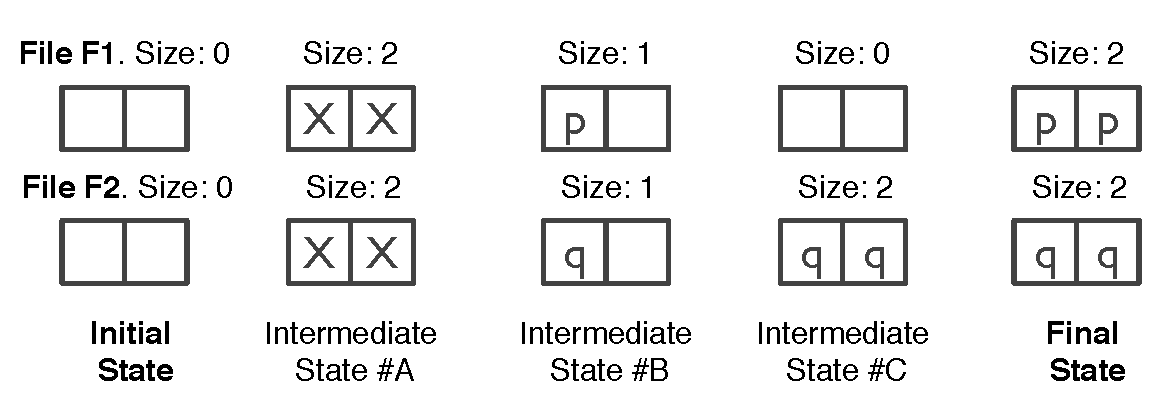
\includegraphics[scale=0.4]{figs/crashstates.eps}
\mycaption{fig-crashstates}{Crash States}{\footnotesize 
The figure shows the initial, final, and some of the intermediate crash states
possible for the workload described in Section~\ref{sec-ppexample} . X
represents garbage data in the files. Intermediate states \#A and \#B represent
different kinds of atomicity violations, while intermediate state \#C
represents an ordering violation.
}
\end{figure}


